\newpage	%--- page 2
\disableTemplate{Lugacover}
%%%--- aebbgtile --> \disableTiling \enableTiling
%%%--- \setTileBgGraphic[scale=0.5]{./img/title_01} % numbers
%%%--- \setTileBgGraphic[scale=0.5]{./img/title_02} % molecule
%%%--- \setTileBgGraphic[scale=0.5]{./img/title_03} % blue lines
%%%--- \setTileBgGraphic[scale=0.5]{./img/title_04} % radio schema
%%%--- \setTileBgGraphic[scale=0.5]{./img/title_05} % blue waves
%%%--- \setTileBgGraphic[scale=0.5]{./img/title_06} % cyan wall 
%%%--- \setTileBgGraphic[scale=0.5]{./img/title_07} % dark blue square
%%%--- \setTileBgGraphic[scale=0.5]{./img/title_08} % gray lines
%%%--- \setTileBgGraphic[scale=0.5]{./img/title_09} % dark cyan wall
%%%--- \setTileBgGraphic[scale=0.5]{./img/title_10} % light wall
%%%--- \setTileBgGraphic[scale=0.5]{./img/title_13} % line left wall
%%%--- \setTileBgGraphic[scale=0.5]{./img/title_14} % math center
%%%--- \setTileBgGraphic[scale=0.5]{./img/title_15} % math spline 
%%%--- \setTileBgGraphic[scale=0.4]{./img/title_16} % securaty lable
%%%--- \setTileBgGraphic[scale=0.35]{./img/title_18} % fractal dark blue
\vglue 25pt
\section{Short Quizzes}
\begin{shortquiz}*[answer] Answer each of the following. Passing is 100\%.
\end{shortquiz}

\vglue 5pt

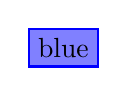
\begin{tikzpicture}[outline/.style={draw=#1,thick,fill=#1!50}]
\node [outline=blue] at (0,0) {blue};
\end{tikzpicture}


\vglue 5pt


\begin{tikzpicture}[rounded corners,ultra thick]
\shade[top color=yellow,bottom color=black] (0,0) rectangle +(2,1);
\shade[left color=yellow,right color=black] (3,0) rectangle +(2,1);
\shadedraw[inner color=yellow,outer color=black,draw=yellow] (6,0)
rectangle +(2,1);
\shade[ball color=green] (9,.5) circle (.5cm);
\end{tikzpicture}

\vglue 5pt

\begin{tikzpicture}[even odd rule,rounded corners=2pt,x=10pt,y=10pt]
\filldraw[fill=examplefill] (0,0) rectangle (1,1)
[xshift=5pt,yshift=5pt] (0,0) rectangle (1,1)
[rotate=30] (-1,-1) rectangle (2,2);
\end{tikzpicture}


\vglue 5pt

\begin{tikzpicture}[->]
\draw (0,0) -- (xyz cs:x=3);
\draw (0,0) -- (xyz cs:y=3);
\draw (0,0) -- (xyz cs:z=3);
\end{tikzpicture}

\begin{tikzpicture}[remember picture,overlay]
\draw [line width=1mm,opacity=.25]
	(current page.center) circle (3cm);
\end{tikzpicture}	

\begin{tikzpicture}[remember picture,overlay]
\node [rotate=60,scale=10,text opacity=0.2]
at (current page.center) {Luga\TeX};
\end{tikzpicture}
